% print no page number
\thispagestyle{empty}

\chapter{Procedural Content Generation}

Το αντικείμενο του Procedural Content Generation (PCG) όπως ορίζεται στο 
\cite{pcgdef} είναι η \textit{Δημιουργία περιεχομένου για ηλεκτρονικά παιχνίδια με την χρήση αλγορίθμων και με την παροχή ελάχιστων ή καθόλου εισόδων από τον χρήστη}. Αποτελεί μια μεγάλη κατηγορία έρευνας και ανάπτυξης για την επιστήμη της πληροφορικής \cite{futureofcontent} και την βιομηχανία των ηλεκτρονικών παιχνιδιών (Video Games). Για συντομία, στο υπόλοιπο κείμενο της εργασίας θα αναφέρετε ως PCG.
\par
Το PCG, όπως και πολλά άλλα αντικείμενα της πληροφορικής, αντιπροσωπεύεται από ιδιαίτερα προβλήματα και περιορισμούς, τόσο στην πολυπλοκότητα των αλγορίθμων όσο και στην αυθεντικότητα και πρωτοτυπία των αποτελεσμάτων.  Ως γνωστικό αντικείμενο της επιστήμης της πληροφορικής, μπορεί να ταξινομηθεί κάτω από την κατηγορία της Τεχνητής Νοημοσύνης. Βασικός στόχος του PCG είναι η δημιουργία αλγορίθμων που μπορούν να προσομοιάσουν την ανθρώπινη δημιουργικότητα και ευφυΐα. Επιπλέον στα προβλήματα και στις προσεγγίσεις επίλυσης παρατηρούμε πολλά κοινά στοιχεία με άλλα πεδία της Τεχνητής Νοημοσύνης.
\par
Όπως έχει παρατηρηθεί και σε πολλά άλλα αντικείμενα της Τεχνητής Νοημοσύνης, έτσι και το PCG είχε μικρή εξάπλωση και χρήση στο ξεκίνημα της επιστήμης. Στη συνέχεια όμως επεκτάθηκε γρήγορα και εδραιώθηκε ως ένας ξεχωριστός τομέας με δικά του προβλήματα, αλγορίθμους και εφαρμογές. Η σταδιακή άνοδος του δεν οφείλεται στις δυνατότητες των αλγορίθμων και της θεωρία πίσω από το αντικείμενο του PCG, αλλά κυρίως στην αδυναμία του υλικού (hardware) των υπολογιστών εκείνων των περιόδων να εφαρμόσουν αλγόριθμους τέτοιας πολυπλοκότητας. Τα τελευταία χρόνια με την ανάπτυξη των δυνατοτήτων των προσωπικών υπολογιστών και των κινητών συσκευών έχει διευρυνθεί η χρήση του PCG για την παραγωγή διαφόρων ειδών περιεχομένου για παιχνίδια (game content). Μαζί με την αύξηση στην χρήση μεθόδων PCG ήρθε και η αύξηση των προβλημάτων που καλείται να επιλύσει.

\begin{figure}[ht]
\centering
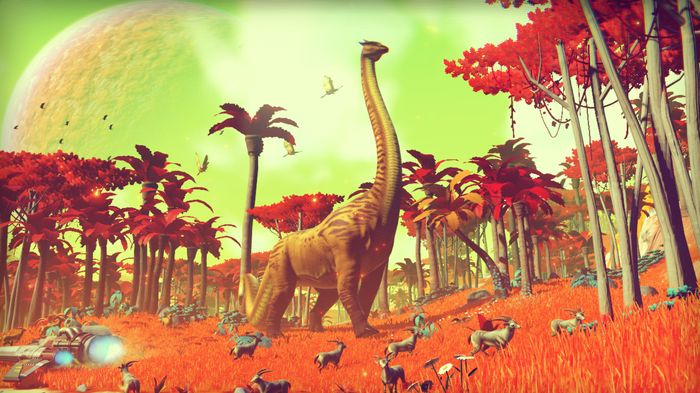
\includegraphics[width=4in]{../images/no-mans-sky.jpg}
\caption{Screenshot από το παιχνίδι No Man's Sky (2016). Οι κόσμοι που δημιουργεί είναι εξολοκλήρου κατασκευασμένοι με τη χρήση ντετερμινιστικών μεθόδων PCG.}
\end{figure}

\section{Περιεχόμενο}
Για να κατανοήσουμε καλύτερη το πεδίο του PCG πρέπει πρώτα να καταλάβουμε τι θεωρείται περιεχόμενο (Game Content) σε ένα παιχνίδι. Ο τομέας του PCG αναφέρεται και έχει χρησιμοποιηθεί σε ηλεκτρονικά παιχνίδια (Video Games), επιτραπέζια παιχνίδια (Board Games), παιχνίδια με κάρτες (Card Games) κ.ά. Το αντικείμενο της συγκεκριμένης εργασίας, επικεντρώνεται στην δημιουργία περιεχομένου για Video Games.

\begin{description}
\item [Game Content] Όπως αναφέρεται και στο όνομα, περιεχόμενο, είναι κάτι που περιέχεται σε ένα παιχνίδι. Αυτός ο ορισμός όμως είναι πολύ γενικός και ευρύς και δεν περιορίζετε μόνο στο περιεχόμενο που αντιστοιχεί στο PCG. Στην βιβλιογραφία μπορούμε να ξεχωρίσουμε συγκεκριμένα είδη περιεχομένου \cite{typesofcontent} που φαίνεται να μπορούν να δημιουργηθούν με μεθόδους PCG. Αυτά είναι:
\end{description}

\begin{itemize}
  \item Γραφικά (Textures)
  \item Επίπεδα (Levels) και χάρτες (Maps)
   \item Αντικείμενα (Items)
   \item Αποστολές (Quests)
   \item Ιστορίες (Stories)
   \item Μουσική (Music)
\end{itemize}

Ο παραπάνω διαχωρισμός γίνεται με βάση το είδος του κάθε περιεχομένου, για παράδειγμα η μουσική ως περιεχόμενο ενός παιχνιδιού, διαφέρει από τα αντικείμενα. Αντίστοιχα οι μεθοδολογίες που έχουν αναπτυχθεί για την παραγωγή μουσικής διαφέρουν από τις μεθόδους που χρησιμοποιούνται για την παραγωγή αντικειμένων. Αυτό βέβαια δεν σημαίνει ότι δεν υπάρχουν κοινοί αλγόριθμοι που μπορούν να εφαρμοστούν σε παραπάνω από ένα είδος με επιτυχία, αντίθετα υπάρχουν πολλοί αλγόριθμοι που έχουν ως βάση έναν πιο γενικό αλγόριθμο και αποτελούν ειδικές εκδόσεις του για το κάθε είδος περιεχομένου.
\par
Ο διαχωρισμός του περιεχομένου βοηθάει στην καλύτερη κατανόηση των ιδιαιτεροτήτων και των περιορισμών που εμφανίζει το κάθε είδος το οποίο οδηγεί στην δημιουργία καλύτερων μεθόδων και αλγορίθμων.

\section{Η χρησιμότητα του PCG}
	Η πρώτη ανάγκη που παρουσιάστηκε και οδήγησε στην υιοθέτηση μεθόδων PCG αφορούσε την μείωση του αποθηκευτικού χώρου που καταλάμβανε ένα παιχνίδι. Το PCG δίνει την δυνατότητα της δημιουργίας του game content μόλις παρουσιαστεί η ανάγκη να χρησιμοποιηθεί ή να εμφανιστεί στον παίκτη. Αυτό σημαίνει ότι δεν χρειάζεται να καταλαμβάνει χώρο στην μνήμη εάν υπάρχει η δυνατότητα της δημιουργίας του ακριβώς την στιγμή που χρειάζεται. Με την μνήμη να αποτελεί έναν διαμοιραζόμενο πόρο μεταξύ των εφαρμογών ακόμα και σήμερα το PCG αποτελεί μια μέθοδο μείωσης του χώρου που καταλαμβάνει ένα παιχνίδι.
\par
	Το PCG έχει επίσης χρησιμότητα από τους καλλιτέχνες και σχεδιαστές διαφόρων παιχνιδιών. Η χρήση PCG για την δημιουργία περιεχομένου το οποίο αν και δεν είναι τέλειο ή αρκετά καλό για το παιχνίδι, δίνεται στους σχεδιαστές οι οποίοι το βελτιώνουν, το αλλάζουν και προσθέτουν στοιχεία ώστε να μπορέσει να προστεθεί με επιτυχία στο παιχνίδι. Με αυτόν τον τρόπο το PCG βοηθάει ανθρώπους με τέτοιους ρόλους στην εργασία τους, δίνοντας του έμπνευση και αναλαμβάνοντας ένα κομμάτι της δουλειάς, με σκοπό αυτοί να μπορέσουν να επικεντρωθούν στα κομμάτια που θα κάνουν το περιεχόμενο πραγματικά εντυπωσιακό. Σε αυτές τις υλοποιήσεις του PCG συνηθίζετε, ο σχεδιαστής να δίνει μέσω διαφόρων εισόδων (inputs) κάποιες παραμέτρους που ορίζουν μια γενική περιγραφή του περιεχομένου που θέλει να δημιουργήσει, όπως το μέγεθος του χάρτη. Στη συνέχεια το PCG δημιουργεί το περιεχόμενο με βάση τις παραμέτρους που πήρε και εμφανίζει το αποτέλεσμα στο σχεδιαστή. Αυτή η διαδικασία μπορεί να επαναληφθεί πολλές φορές μέχρι ο σχεδιαστής να είναι ικανοποιημένος με το παραγόμενο αποτέλεσμα.  \cite{pcgieee}
\par
	Μια επίσης πολύ σημαντική ανάγκη που καλύπτει, εν μέρη, το PCG είναι η δημιουργία ενός παιχνιδιού που δεν τελειώνει ποτέ (endless). Αντίθετα με την συνεχή παραγωγή πρωτότυπου περιεχομένου, ένα παιχνίδι μπορεί να συνεχίζετε επ’ άπειρον, προσφέροντας αμέτρητες ώρες διασκέδασης στους παίκτες. Πολλά παιχνίδια έχουν επιχειρήσει να υλοποιήσουν αυτό το χαρακτηριστικό, κάποια με μεγάλη επιτυχία και κάποια με το αντίθετο αποτέλεσμα. Ένα από τα μεγαλύτερα προβλήματα που αντιμετωπίζουν οι υλοποιήσεις του PCG είναι η επαναληψιμότητα και η μονοτονία, όπως θα αναλυθεί και παρακάτω. Η έλλειψη της μονοτονίας είναι ένα από τα πιο σημαντικά κριτήρια για την επιτυχία ενός endless video game.
\par
	Τέλος, μια ανάγκη που έχει προκύψει τα τελευταία χρόνια στον χώρο των παιχνιδιών και συνδέετε με μια ακόμα περιοχή της Τεχνητής Νοημοσύνης στα παιχνίδια είναι η εξατομίκευση περιεχομένου, ή personalized content. Αναφέρεται στην δημιουργία περιεχομένου που είναι σχεδιασμένο για τις προτιμήσεις και τις ανάγκες του κάθε παίκτη.

\section{Παιχνίδια που χρησιμοποιούν PCG}

Από την πρώτη στιγμή που ξεκίνησε η διάδοση των Video Games φάνηκε η ανάγκη για την αυτόματη και αυτόνομη δημιουργία   \textit{σωστού} περιεχομένου. Κάποια από τα παιχνίδια που εφάρμοσαν με μεγάλη επιτυχία μεθόδους PCG είναι:

\begin{description}
\item [Rogue (\textbf{1980})] Ένα από τα πρώτα παιχνίδια που εφάρμοσε PCG για την αυτόματη δημιουργία επιπέδων (\textbf{levels}). Το Rogue ενέπνευσε την δημιουργία πολλών παιχνιδιών με αντίστοιχες δυνατότητες και PCG μεθόδους. \cite{rogue}

\item [Spore (\textbf{2008})] Το Spore είναι ένα παιχνίδι προσημείωσης και στρατηγικής που χρησιμοποιεί PCG για την δημιουργία πλασμάτων και αντικειμένων. Οι αλγόριθμοι του Spore, συνδυάζουν απλά σχήματα και αντικείμενα για να δημιουργήσουν μεγαλύτερα και πιο πολύπλοκα πλάσματα με βάση διάφορους κανόνες και περιορισμούς. \cite{spore} 

\item [No Man's Sky (\textbf{2016})] Ένα από τα πιο σημαντικά παραδείγματα για τις δυνατότητες του PCG είναι το παιχνίδι no Man's Sky. Το θέμα του παιχνιδιού είναι η εξερεύνηση του διαστήματος και η επιβίωση σε ξένους πλανήτες. Το παιχνίδι δημιουργεί σχεδόν ολόκληρο τον κόσμο με PCG, δηλαδή τους πλανήτες, τα αστέρια, τα φυτά, τα ζώα και τα encounters του παίκτη με τη χρήση ντετερμινιστικών αλγορίθμων PCG. Η αποδοχή του παιχνιδιού από το κοινό ήταν μέτρια. Οι δημιουργοί είχαν υποσχεθεί έναν απέραντο κόσμο γεμάτο περιεχόμενο και οι παίκτες παρατήρησαν ότι το τελικό αποτέλεσμα ήταν μονότονο και επαναλαμβανόμενο, κάτι που τους δημιούργησε άσχημες εντυπώσεις.  \cite{nomanssky}
\end{description}

\section{Προβλήματα του PCG}
Όπως αναφέρθηκε και παραπάνω, το PCG δεν αποτελεί μια τέλεια και ολοκληρωμένη λύση για να τα προβλήματα που καλείται να αντιμετωπίσει. Αντίθετα οι υλοποιήσεις του PCG πρέπει να λαμβάνουν υπόψη τα καινούργια προβλήματα και περιορισμούς που δημιουργούνται με την χρήση των PCG αλγορίθμων. \cite{challenges} \cite{desirableproperties}

\begin{description}
\item [Επαναληψιμότητα - Μονοτονία] Ένα από τα πιο σημαντικά θέματα είναι η ποικιλία και μοναδικότητα του παραγόμενου περιεχομένου. Όπως αναλύθηκε και παραπάνω, σε πολλές περιπτώσεις το παραγόμενο περιεχόμενο είναι πολύ μονότονο, μοτίβα φαίνονται να επαναλαμβάνονται και κατά συνέπεια το αποτέλεσμα δίνει στον χρήστη την αντίθετη εντύπωση από την επιθυμητή. Οι λόγοι που συμβαίνει αυτό είναι πολλοί και σχετίζονται με το είδος του αλγόριθμου που χρησιμοποιείται κάθε φορά, τις παραμέτρους που δίνονται και τα βασικά assets που χρησιμοποιεί για να δημιουργήσει το περιεχόμενο.

\item [Ταχύτητα - πολυπλοκότητα] Πολλοί αλγόριθμοι PCG πρέπει να είναι σε θέση να λειτουργούν σε πολύ λίγο χρόνο και με περιορισμένους πόρους. Σε ένα ηλεκτρονικό παιχνίδι υπάρχουν πολλά κομμάτια που πρέπει να δουλεύουν ταυτόχρονα, όπως τα γραφικά, το UI, το σύστημα κανόνων για την προσομοίωση της φυσικής στον κόσμο του παιχνιδιού κ.ά. Συνεπώς το σύστημα του AI που περιέχει και το PCG δεν μπορεί να καταλαμβάνει πολλούς πόρους ή να αργεί να ανταποκριθεί γιατί το παιχνίδι θα φαίνεται να κολλάει ή να μην δουλεύει όπως πρέπει. Αυτό σημαίνει ότι οι αλγόριθμοι που υλοποιούν το PCG πρέπει να έχουν συγκεκριμένη χρονική και χωρική πολυπλοκότητα και να μην την ξεπερνάνε.

\item [Playability] Μπορεί να έχουμε σχεδιάσει τον τέλειο αλγόριθμο PCG που χρησιμοποιεί ελάχιστους πόρους του συστήματος και δημιουργεί μοναδικά επίπεδα για το 2D platformer παιχνίδι μας αλλά ένα στα τρία επίπεδα να μην έχουν είσοδο.Αυτό σημαίνει ότι ο παίκτης δεν θα μπορέσει να το επισκεφτεί ποτέ, ή θα βρεθεί παγιδευμένος μέσα του χωρίς κάποιο τρόπο να προχωρήσει το παιχνίδι. Αυτό φυσικά είναι κάτι που δεν θέλουμε σε καμία περίπτωση να συμβεί. Για αυτό το λόγο πρέπει να ορίσουμε τι θεωρείται "playable" περιεχόμενο και τι "unplayable".
 
\end{description}


\section{Επιθυμητά Χαρακτηριστικά του PCG}
Με βάση τα παραπάνω στοιχεία μπορούμε να αναλύσουμε ένα σύνολο από επιθυμητά χαρακτηριστικά που θέλουμε να έχει κάθε σύστημα PCG ώστε να διασφαλίσουμε την σωστή και αρμονική λειτουργία του μέσα στο παιχνίδι.  \cite{challenges} \cite{desirableproperties}

\subsection{Ταχύτητα - Πολυπλοκότητα} Όπως είδαμε και στο 1.4 ένα μεγάλο θέμα για κάθε παιχνίδι είναι η διαχείριση και κατανομή των πόρων στα επιμέρους συστήματα του. Το σύστημα του AI, που περιέχει και το υποσύστημα του PCG πρέπει να περιορίσει την πολυπλοκότητα των αλγορίθμων του, χρονικά και χωρικά, ώστε να ανταποκρίνονται στους διαθέσιμους πόρους. Αυτός ο περιορισμός είναι ιδιαίτερα σημαντικός για την επιτυχία του παιχνιδιού καθώς η εμπειρία του παίκτη σχετίζεται άμεσα με την πόσο γρήγορα και σωστά ανταποκρίνεται το παιχνίδι. 
\par
Εάν το αλγόριθμος που δημιουργεί όπλα ειδικά για τον παίκτη (personalized) αργήσει να ολοκληρώσει την λειτουργία του, θα δημιουργηθεί στον παίκτη η εντύπωση ότι το παιχνίδι έχει "κολλήσει" και δεν ανταποκρίνεται. Αυτό θα έχει ως συνέπεια να πάρει μια αρνητική εμπειρία από το παιχνίδι. Αντίθετα, τα παιχνίδια που καταφέρνουν να ανταποκρίνονται άμεσα σε κάθε εντολή του παίκτη λαμβάνουν πολύ θετικά σχόλια τόσο από το κοινό όσο και από κριτικούς του χώρου.

\subsection{Δημιουργικότητα - πρωτοτυπία} Το ιδανικό σύστημα PCG θα δημιουργεί περιεχόμενο αντίστοιχο με το περιεχόμενο που δημιουργεί ένας σχεδιαστής (designer) σε θέμα πρωτοτυπίας και δημιουργικότητας. Όπως είδαμε από τα παραδείγματα παραπάνω αυτό δεν ισχύει καθολικά ή στον βαθμό που θέλουμε πάντα. Είναι πολύ δύσκολη η καταγραφή και έκφραση της δημιουργικότητας με όρους που μπορεί να καταλάβει ένας αλγόριθμος. Αποτελεί ακόμα ένα ανοιχτό πρόβλημα στον χώρο της Τεχνητής Νοημοσύνης και επηρεάζει άμεσα τα αποτελέσματα του PCG.
\par
Ωστόσο έχουν γίνει πολλές προσπάθειες και βελτιώσεις σε αυτό το χαρακτηριστικό του PCG ιδιαίτερα με την χρήση βαθιών νευρωνικών δικτύων. Επίσης το παραγόμενο περιεχόμενο θέλουμε να δίνει την εντύπωση ότι δεν δημιουργήθηκε από κάποιον αλγόριθμο, αλλά από κάποιον άνθρωπο. Αυτό το χαρακτηριστικό είναι πολύ δύσκολο να επιτευχθεί. Με την αύξηση της χρήσης του PCG στα παιχνίδια, οι παίκτες "έμαθαν" να ξεχωρίζουν το περιεχόμενο που παράγεται από αλγορίθμους και να προσπαθούν σε πολλές περιπτώσεις να το χρησιμοποιήσουν προς όφελος τους για να "παρακάμψουν" κανόνες του παιχνιδιού.
\par
Για παράδειγμα στο παιχνίδι Mount and Blade II Bannerlord \cite{bannerlord} υπάρχει η πιθανότητα το παιχνίδι να δημιουργήσει μάχες κατά την διάρκεια αποστολών για να τις κάνει πιο δύσκολες και ενδιαφέρουσες. Οι παίκτες γνωρίζοντας ότι το σύστημα του PCG υπολογίζει την πιθανότητα μάχης εκείνη την στιγμή, μπορούν να φορτώσουν το παιχνίδι σε κάποια προηγούμενη στιγμή και όταν φτάσουν στο σημείο της μάχης, το σύστημα να επαναϋπολογίσει την πιθανότητα, αυτή την φορά βγάζοντας αρνητική πιθανότητα μάχης. 

\subsection{Αξιοπιστία} H αξιοπιστία του παραγόμενου περιεχομένου συνδέεται άμεσα με μια πολύ απλή ερώτηση: Είναι playable? Μπορεί δηλαδή το περιεχόμενο που παράχθηκε να προστεθεί στο παιχνίδι και να το χρησιμοποιήσει ο παίκτης ή δημιουργεί προβλήματα; Για παράδειγμα ένα όπλο χωρίς σκανδάλη ή χωρίς την λειτουργικότητα της σκανδάλης είναι άχρηστο. Εκτός από το αν είναι χρήσιμο, το περιεχόμενο θα πρέπει να μην "σπάει" το παιχνίδι. Δηλαδή να μην παγιδεύει το παίκτη σε καταστάσεις από τις οποίες δεν μπορεί να συνεχίσει την πρόοδο του ή να του δίνει πλεονεκτήματα που σπάνε τους κανόνες του παιχνιδιού.
\par
Για τον έλεγχο της αξιοπιστίας του παραγόμενου περιεχομένου υπάρχουν οι τα συστήματα αξιολόγησης (evaluators). Είναι αλγόριθμοι του συστήματος PCG και "αποφασίζουν" εάν το περιεχόμενο που παράχθηκε είναι playable ή όχι. Εάν το αξιολογήσουν ως unplayable, ο PCG αλγόριθμος πρέπει να δημιουργεί καινούργιο περιεχόμενο μέχρι κάποιο να περάσει την αξιολόγηση αξιοπιστίας.

\subsection{Παραμετροποίηση} Σε όλους τους αλγόριθμους PCG δίνονται κάποιοι παράμετροι ως είσοδοι. Από αυτές τις παραμέτρους εξαρτώνται συγκεκριμένα χαρακτηριστικά που θα έχει το παραγόμενο αποτέλεσμα. Αυτή η δυνατότητα είναι πολύ σημαντική για τα συστήματα PCG που χτίζονται για να χρησιμοποιηθούν από τους designers του παιχνιδιού. Επιπλέον, αυτές οι είσοδοι καθορίζουν πόσο ντετερμινιστικό είναι ένα σύστημα PCG.
\par
Για παράδειγμα στο παιχνίδι Oxygen Not Included (2019), ένα παιχνίδι προσομοίωσης και επιβίωσης, δημιουργείται το επίπεδο στο οποίο ο παίκτης θα πρέπει να χτίσει την βάση του, χρησιμοποιώντας μια αλφαριθμητική μοναδική τιμή, ή όπως λέγετε στην επιστήμη της κρυπτογραφίας (seed). Αυτό το seed μπορεί να παραχθεί τυχαία από το παιχνίδι ή να το παρέχει στο σύστημα ως είσοδο ο παίκτης. Αυτή η δυνατότητα έχει ως αποτέλεσμα οι παίκτες να μπορούν να βρουν και να ανταλλάξουν seeds για επίπεδα που τους φάνηκαν πολύ ευνοϊκά ή πολύ δύσκολα. Το συγκεκριμένο χαρακτηριστικό παρατηρήθηκε να βελτιώνει την εμπειρία των παικτών με το παιχνίδι καθώς δημιουργήθηκε μια κοινότητα παικτών(community) που μοιραζόντουσαν seeds από επίπεδα με άλλους παίκτες και σύγκριναν τις εμπειρίες και τις επιδόσεις τους. \cite{oxygennotincluded}

% leave 60mm empty space below
\vspace{60mm}

\section{Procedural Content Generation για 2D επίπεδα}

Ένας τομέας με πολλές εφαρμογές του PCG είναι τα παιχνίδια δύο διαστάσεων (2D) και η δημιουργία επιπέδων (levels/dungeon) για αυτά. Ένα τέτοιο επίπεδο μπορεί να οριστεί ως ένας 2D χώρος, ο οποίος περιέχει δωμάτια ή τμήματα, χωρισμένα με διαχωριστικά ή άλλα εμπόδια. Ο παίκτης μπορεί να περιηγηθεί στο επίπεδο με βάση τους κανόνες του κάθε παιχνιδιού, είτε μέσα από πόρτες και ανοίγματα ή ανοίγοντας τρύπες στα διαχωριστικά. Καθώς εξερευνάει μπορεί να συναντήσει αντικείμενα, εχθρούς, κρυφά περάσματα κ.ά. 
\par
Σε αυτή την εργασία αναπτύχθηκαν αλγόριθμοι και μοντέλα για την δημιουργία τέτοιων επιπέδων, συνεπώς είναι σημαντικό να αναλυθούν οι διάφοροι περιορισμοί και ιδιαιτερότητες αυτού του τομέα, καθώς και αντιπροσωπευτικές μέθοδοι και τα χαρακτηριστικά τους.
\par
Η μελέτη και επιλογή αυτού του τομέα είναι ιδιαίτερα διαδεδομένη στην επιστημονική κοινότητα του PCG καθώς προσφέρει ένα χώρο αναζήτησης(search space) που μπορεί εύκολα να αναπαρασταθεί και να αποθηκευτεί σε διάφορες μορφές. Επίσης είναι εύκολη η αξιολόγηση και η δοκιμή τέτοιου περιεχομένου όπως θα αναλυθεί και παρακάτω.

\subsection{Εισαγωγή}
Όπως περιγράφετε και στα \cite{pcgieee} \cite{pcgig}, το PCG για την δημιουργία τέτοιων επιπέδων περιέχει την δημιουργία της τοπολογίας, της γεωμετρίας και των αντικειμένων του επιπέδου. Στο \cite{pcgig} γίνετε μια ανάλυση ενός συστήματος PCG σε τρία βασικά στοιχεία:

\begin{description}
  \item[$\bullet$ Μοντέλο αναπαράστασης] Αποτελεί μια απλοποιημένη και γενική αναπαράσταση ενός επιπέδου.
  \item[$\bullet$ Μέθοδο δημιουργίας του μοντέλου αναπαράστασης] Ο αλγόριθμος που μετατρέπει τα επίπεδα στο \textit{μοντέλο αναπαράστασης} όπως έχει οριστεί. 
    \item[$\bullet$ Μέθοδο δημιουργίας του επιπέδου από το μοντέλο αναπαράστασης] Ο αλγόριθμος που αναλαμβάνει να δημιουργήσει το επίπεδο στον χώρο του παιχνιδιού με βάση το \textit{μοντέλο αναπαράστασης} που δημιούργησε η \textit{μέθοδος δημιουργίας}. Αυτό είναι το αποτέλεσμα που θα παρουσιαστεί στον τελικό χρήστη του συστήματος.
\end{description}

Παρακάτω συνοψίζονται μερικές από τις πιο γνωστές οικογένειες αλγορίθμων PCG για 2D επίπεδα:

\begin{description}
  \item[$\bullet$ PCG με διαχωρισμό χώρου (Space Partitioning)] 
  \item[$\bullet$ PCG με την χρήση πρακτόρων (Agent-based)]
    \item[$\bullet$ PCG με Cellular Automata] 
    \item[$\bullet$ PCG με τη χρήση γραμματικών (Generative Grammars)] 
\end{description}

\subsection{Space Partitioning}
Αυτή η ομάδα αλγορίθμων χρησιμοποιείται και σε άλλες περιοχές του game development όπως τα γραφικά, οπότε οι μεθοδολογίες και οι δομές δεδομένων είναι γνωστά στους σχεδιαστές και προγραμματιστές παιχνιδιών. Όπως περιγράφει και το όνομα της, εκτελεί έναν διαχωρισμό του χώρου σε υποχώρους. Αυτό μπορεί να χρησιμοποιηθεί στο PCG για την δημιουργία δωματίων και διαδρόμων μέσα σε ένα  επίπεδο. \cite{pcgspacepart}
\par
Ένας αλγόριθμος που χρησιμοποιείται πολύ σε υλοποιήσεις space partitioning είναι ο Binary Space Partitioning (BSP) \cite{bsp} και παραλλαγές του όπως o Quadtree space partitioning και ο Octree space partitioning. Θα αναλύσουμε τον βασικό αλγόριθμο του BSP, αναλυτικές περιγραφές για τους quadree και octree μπορούν να βρεθούν εδώ \cite{octree}.

\begin{description}
  \item[$\bullet$ Binary Space Partitioning (BSP)]
  Ο αλγόριθμος είναι αναδρομικός και χτίζει το επίπεδο ιεραρχικά χρησιμοποιώντας ως δομή δεδομένων ένα Δυαδικό Δέντρο (Binary Tree). Στο αρχικό στοιχείο (root node ) του Binary Tree περιέχεται "ολόκληρο" το επίπεδο. Στην πρώτη αναδρομή, το επιλεγμένο στοιχείο (node), το root σε αυτή την περίπτωση χωρίζεται σε δύο τμήματα με κάποιον ορισμένο διαχωρισμό, για παράδειγμα κάθετα. Αυτά τα δύο κομμάτια προστίθενται ως παιδιά (child nodes) στο root node και στη συνέχεια ο αλγόριθμος καλείται για κάθε ένα από τα παιδιά.
  \par
  Ο αλγόριθμος σταματάει όταν φτάσει σε κάποια προορισμένη τερματική συνθήκη, για παράδειγμα το μέγιστο βάθος δέντρου ή μόλις τελειώσουν τα nodes που υπάρχουν για διαχωρισμό. Για να προστεθεί τυχαιότητα στον αλγόριθμο, άρα και διαφοροποίηση στα παραγόμενα επίπεδα σε κάθε εκτέλεση, μπορεί να αποδοθεί μια πιθανότητα διαχωρισμού σε κάθε node. Αν η πιθανότητα είναι κάτω από ένα ορισμένο κατώφλι να μην γίνετε διαχωρισμός αυτού του node. Επιπλέον το κατώφλι μπορεί να διαμορφώνεται ανάλογα με το μέγεθος του παραγόμενου επιπέδου ή το βάθος που βρίσκεται αυτή τη στιγμή ο αλγόριθμος.
  \par 
  Η εισαγωγή και δοκιμή τέτοιων παραμέτρων είναι ένα μεγάλο κομμάτι της υλοποίησης, και παίζει καθοριστικό ρόλο στο τελικό αποτέλεσμα. Τέτοιου είδους παράμετροι μπορούν να χρησιμοποιηθούν από τους σχεδιαστές για να παράγουν διαφόρων ειδών επίπεδα.
\end{description}

Ένα σημαντικό χαρακτηριστικό αυτής της οικογένειας αλγορίθμων, είναι ότι δημιουργεί επίπεδα με δωμάτια τα οποία δεν υπερκαλύπτουν άλλα δωμάτια. Αυτό συμβαίνει προφανώς επειδή ένα δωμάτιο προέρχεται από τον διαχωρισμό ενός μεγαλύτερου δωματίου σε συγκεκριμένα τμήματα, το κάθε ένα εντελώς ξεχωριστό από το άλλο.

\subsection{Agent-based}
Όπως αναφέρει και το όνομα αυτής της οικογένειας, η δημιουργία του επιπέδου γίνετε μέσω ενός πράκτορα \cite{agents}. Οι πράκτορες αντίστοιχα με το Space Partitioning είναι συχνά χρησιμοποιούμενοι αλγόριθμοι και από άλλα κομμάτια του παιχνιδιού, όπως για παράδειγμα για την συμπεριφορά χαρακτήρων που δεν ελέγχει ο παίκτης (NPCs).
\par
Σε αντίθεση με το Space Partitioning, οι Agent-Based προσεγγίσεις δεν βλέπουν ολόκληρο τον χώρο καθώς εκτελούνται, αλλά μόνο ένα συγκεκριμένο πεδίο γύρω από τον πράκτορα ανάλογα με τις δυνατότητες που του έχουμε δώσει. Αυτή η διαφορά, κάνει τα αποτελέσματα του Agent-Based PCG να είναι πιο χαοτικά και τυχαία από τα οργανωμένα επίπεδα που αναλύσαμε παραπάνω.
\par
Για την δημιουργία ενός τέτοιου αλγόριθμου πρέπει να οριστεί μια συμπεριφορά για τον πράκτορα και στη συνέχεια να τον "ελευθερώσουμε" στο επίπεδο που θέλουμε να δημιουργήσει. Ο πράκτορας θα "περιπλανιέται" (wander) στον χώρο και με βάση παραμέτρους της συμπεριφορά του θα το αλλάζει με σκοπό να δημιουργήσει έναν χώρο που να είναι αποδεκτός ως επίπεδο στο παιχνίδι μας.
\par
Για παράδειγμα μπορούμε να ορίσουμε ένα State Machine ως την συμπεριφορά του πράκτορα μας το οποίο αποτελείται από τα ακόλουθα States:
\begin{description}
  \item[$\bullet$ Περιπλάνηση (Wandering)] Όταν ο πράκτορας βρίσκεται σε αυτό το State, περιπλανιέται στο χώρο σε μια ευθεία. Με μια αυξανόμενη πιθανότητα μετά από κάθε κίνηση σε αυτό το State ο πράκτορας μπορεί να μεταβεί στο State Turn ή στο State Room Placement.
  \item[$\bullet$ Στροφή (Turn)] Μόλις βρεθεί σε αυτό το State, ο πράκτορας επιλέγει μια καινούργια κατεύθυνση και ξεκινάει να κινείται προς αυτήν επιστρέφοντας στο State του Wandering. 
    \item[$\bullet$ Τοποθέτηση δωματίου (Room placement)] Σε αυτό το State, ο πράκτορας επιλέγει ένα δωμάτιο τυχαίων διαστάσεων και το τοποθετεί μπροστά του. Στη συνέχεια επιστρέφει στο State Wandering.
\end{description}
Με αυτά τα τρία πολύ απλά States, και τις παραμέτρους που επηρεάζουν τις μεταβάσεις και το μέγεθος των δωματίων έχουμε ορίσει έναν πράκτορα που μπορεί να δημιουργήσει επίπεδα με τυχαία διασκορπισμένα δωμάτια. Αντίστοιχα με το Space Partitioning, αυτές οι παράμετροι που καθορίζουν τις μεταβάσεις των States μπορούν να χρησιμοποιηθούν από designers για να δημιουργούν επίπεδα με τις παραμέτρους που τους βολεύουν.
\par
Ένα μεγάλο πλεονέκτημα των Agent-based αλγορίθμων είναι ότι είναι παραλληλοποιήσιμοι. Δηλαδή μπορούμε να αρχικοποιήσουμε ένα επίπεδο με τέσσερις πράκτορες ώστε να έχουμε πιο γρήγορη δημιουργία και διαφορετικό αποτέλεσμα καθώς η εκτέλεση τεσσάρων πρακτόρων θα δημιουργήσει πολύ διαφορετικό περιεχόμενο απ ότι ο ένας πράκτορας. Αυτή η προσέγγιση συνοδεύεται από επιπλέον λογική στη συμπεριφορά των πρακτόρων για την συνεργασία ή αποφυγή της επικάλυψης του έργου του ενός πράκτορα από τους άλλους.

\subsection{Cellular Automata}
Τα Cellular Automata (ενικός: Cellular Automaton) \cite{cellular} έχουν χρησιμοποιηθεί πέρα από την επιστήμη της Πληροφορικής, από την Φυσική και την Βιολογία για να προσομειώσουν μοντέλα ανάπτυξης και φυσικά φαινόμενα. Στον τομέα του PCG έχουν χρησιμοποιηθεί με μεγάλη επιτυχία για την δημιουργία δωματίων με πολύ φυσική σπηλαιώδη τοπολογία.
\par
Το περιβάλλον δημιουργίας του επιπέδου αποτελεί ένα NxM επίπεδο (grid) αποτελούμενο από κελιά (cells), ένα σύνολο κανόνων μετάβασης και ένα σύνολο καταστάσεων. Αυτά τα τρία στοιχεία είναι αρκετά για να οριστεί μια υλοποίηση με Cellular Automata. 
\par
 Ο αλγόριθμος των Cellular Automata εκτελείται σε επαναλήψεις, κάνοντας κάθε φορά αλλαγές μέχρι να φτάσει στο τελικό αποτέλεσμα του επιπέδου. Αυτό γίνετε μόλις φτάσει σε κάποια τερματική συνθήκη ή μόλις σταματήσει να καταγράφει αρκετές μεταβολές στις καταστάσεις των cells.
\begin{description}
  \item[$\bullet$ Grid] Το NxM grid αντιπροσωπεύει το επίπεδο που θέλουμε να υλοποιήσουμε, όπου το κάθε στοιχείο του ονομάζετε cell. Αρχικά για να μπορέσει να λειτουργήσει ο αλγόριθμος πρέπει τα cells του grid να λάβουν αρχικές τιμές από τις διαθέσιμες καταστάσεις. Αυτό συνήθως γίνετε με τυχαία ανάθεση τιμών η οποία μπορεί να ακολουθεί κάποια κατανομή που θέλουμε να έχουν τα cells στο επίπεδο.
  \item[$\bullet$ Κανόνες μετάβασης (Transition Rules)] Αυτοί οι κανόνες εφαρμόζονται σε κάθε επανάληψη σειριακά σε όλα τα cells του grid. Με βάση αυτούς τους κανόνες, σε συνδυασμό με την "γειτονιά" του cell αποφασίζετε αν θα αλλάξει η κατάσταση του και σε ποια κατάσταση θα μεταβεί.
    \item[$\bullet$ Σύνολο καταστάσεων (Set of States)] Περιλαμβάνει όλες τις δυνατές καταστάσεις που μπορεί να έχει ένα cell ανά πάσα στιγμή. Μόνο μία κατάσταση μπορεί να ανατεθεί στο cell κάθε φορά.
\end{description}
\par
Πολύ σημαντική παράμετρος για τα αποτελέσματα του αλγορίθμου είναι η "γειτονιά" του cell. Ως γειτονιά ορίζεται το σύνολο των cells που είναι κοντά στο cell που εξετάζουμε και επηρεάζουν την κατάσταση στην οποία θα μεταβεί. Για ένα μονοδιάστατο cell, γειτονιά ορίζετε ως τα cells που βρίσκονται δεξιά και αριστερά του σε X απόσταση. Αν το X = 1 τότε παίρνουμε μόνο τα cells που είναι ακριβώς δίπλα του. Σε δισδιάστατα cells υπάρχουν δύο γειτονιές ορισμένες στην βιβλιογραφία.
\begin{description}
  \item[$\bullet$ Moore Neighborhood] Η Moore Neighborhood μοιάζει με σταυρό, περιλαμβάνει τα cells που είναι πάνω, κάτω, δεξιά και αριστερά του cell που εξετάζουμε. 
    \item[$\bullet$ Von Neumann Neighborhood] Αυτή η γειτονιά περιλαμβάνει όλα τα cells που έχει και η Moore Neighborhood και τα cells που βρίσκονται διαγωνίως του cell που εξετάζουμε.
\end{description}
Και οι δύο γειτονιές, αντίστοιχα με τη μονοδιάστατη γειτονιά μπορούν να εκτείνονται κατά X cells μακρυά από το cell που εξετάζουμε. Δεν είναι κανόνας αλλά συνηθίζεται στις υλοποιήσεις το X να είναι 1.
\par
Σε αυτή την εργασία χρησιμοποιήθηκαν μέθοδοι Cellular Automata σε συνδυασμό με το Space Partitioning όπως θα αναλυθεί στη συνέχεια.


\subsection{Generative Grammars}
Οι γραμματικές όπως ορίζονται στον τομέα του Game Development και γενικότερα στην επιστήμη της Πληροφορικής \cite{grammars}, αποτελούνται από μεταβλητές και κανόνες. Οι μεταβλητές αντιπροσωπεύονται από μικρά λατινικά γράμματα και οι κανόνες από κεφαλαία. Οι κανόνες αποτελούν κανόνες μετατροπής ενός ή περισσότερων κεφαλαίων συμβόλων σε μια ακολουθία από μικρά και κεφαλαία σύμβολα αντίστοιχα.
\par 
Για παράδειγμα μπορούμε να ορίσουμε μια γραμματική με μεταβλητές το σύνολο {a, b} και κανόνες το σύνολο {Α -> a, B -> Ab}. Συνεπώς αν η αρχική μας κατάσταση είναι η {ΑΒ} μόλις εφαρμόσουμε τους κανόνες μετατροπής θα έχουμε την κατάσταση {ΑΒ} -> {aΑb}. Αντίστοιχα μπορούμε να συνεχίσουμε να εφαρμόζουμε τους κανόνες μέχρι να ικανοποιήσουμε κάποια τερματική συνθήκη ή να έχουμε μετατρέψει όλα τα κεφαλαία σύμβολα σε μικρά.
\par
Αυτού του είδους οι γραμματικές είναι πολύ αποτελεσματικές στην δημιουργία φυτών, όπως δέντρα, θάμνους κ.ά. Συνεπώς η χρήση τους είναι ιδιαίτερα γνωστή στον κόσμο του game development αντίστοιχα με τους προηγούμενους αλγόριθμους. Γενικά παρατηρούμε ότι πολλοί αλγόριθμοι έχουν εφαρμογή σε περισσότερους από έναν τομέα.
\par
Για την δημιουργία ενός επιπέδου με την χρήση γραμματικών η διαδικασία είναι λίγο διαφορετική από αυτές που έχουμε δει ως τώρα. Μια ακόμα χρήση των Generative Grammars είναι η δημιουργία αποστολών (Quests). Επειδή υπάρχει μια λογική ακολουθία στην εξέλιξη μιας αποστολής, για παράδειγμα:
\newline
Νίκησε τον εχθρό στο δωμάτιο 1 -> Πάρε το κλειδί που κουβαλούσε -> Ξεκλείδωσε το δωμάτιο 2 
\newline
Η χρήση γραμματικών για την δημιουργία γράφων που αντιπροσωπεύουν αποστολές σε ένα παιχνίδι είναι μια μέθοδος που χρησιμοποιείται. Κατά συνέπεια, εφόσον έχουμε τον συνδεδεμένο γράφο της αποστολής μπορούμε να υλοποιήσουμε έναν αντίστοιχο γράφο που να αντιπροσωπεύει το επίπεδο που θα εκτελεστεί αυτή η αποστολή. Μπορούμε να βάλουμε επιπλέον δωμάτια και διαδρόμους ώστε να φαίνεται πιο "γεμάτο" το επίπεδο αλλά πρέπει να είμαστε προσεκτικοί και να ακολουθήσουμε ακριβώς την ιεραρχία του γράφου της αποστολής ώστε να μην καταλήξουμε με κάποιο επίπεδο που δεν μπορεί να εκτελεστεί η αποστολή. Ένα τέτοιο παράδειγμα επιπέδου θα ήταν εάν στο παραπάνω σενάριο, το δωμάτιο 1 ήταν μετά το δωμάτιο 2 και δεν υπήρχε τρόπος για τον χρήστη να τον φτάσει παρά μόνο μέσω του δωματίου 2.
\par
Βλέπουμε εδώ μια πιο γενική και αφηρημένη αναπαράσταση ενός επιπέδου, το οποίο έχει διάφορα πλεονεκτήματα. Συγκεκριμένα δίνει μια μεγαλύτερη ελευθερία για τυχαιότητα αλλά επειδή υπάρχει μια συγκεκριμένη ιεραρχία κάποιων δωματίων δεν φαίνεται εντελώς τυχαίο στον παίκτη. Αντίθετα μπορεί να υποθέσει ότι κάποιος άνθρωπος το σχεδίασε ώστε να έχει μια λογική συνοχή.
\par
Επιπλέον επειδή οι αναπαραστάσεις δεν είναι στενά συνδεδεμένες με το παιχνίδι και τη δομή του μπορούν να μεταφερθούν αυτούσιες σε κάποιο άλλο παιχνίδι αντίστοιχου τύπου και να αναπαρασταθούν σε αυτό. Προσφέρει δηλαδή μια πιο γενική και επαναχρησιμοποιούμενη αναπαράσταση από τις προηγούμενες μεθόδους.


\section{Αξιολόγηση (Evaluation)}
Είδαμε μερικούς από τους αλγόριθμους που μπορούν να χρησιμοποιηθούν για την δημιουργία περιεχομένου. Υπάρχουν πολλοί περισσότεροι, ο καθένας με τις παραλλαγές του. Συμπεραίνουμε ότι είναι πολύ εύκολο να δημιουργήσουμε περιεχόμενο, το δύσκολο κομμάτι του PCG είναι η δημιουργία \textbf{καλού} περιεχομένου. Σε αυτή την ενότητα θα αναλύσουμε πως γίνετε την αξιολόγηση PCG συστημάτων με τη χρήση άλλων συστημάτων, των Evaluators. \cite{pcgevaluation}

\subsection{Πόσο σημαντική είναι η αξιολόγηση}
Τα νούμερα και οι μετρήσεις αποτελούν τις βάσεις κάθε επιστήμης. Αυτά δείχνουν την πορεία ενός αλγορίθμου από την αρχική του σχεδίαση μέχρι την τελευταία του αλλαγή. Αποδίδουν την ιστορικότητα και την βελτίωση ή χειροτέρευση μιας κατάστασης με πολύ συμπυκνωμένο και κατανοητό τρόπο για τους ανθρώπους που την παρακολουθούν. Αντίστοιχα και στην επιστήμη του PCG χρειαζόμαστε μεθόδους για να μετράμε την πορεία και την απόδοση του συστήματος. Αυτή την εργασία την αναλαμβάνουν οι Evaluators όπως έχει ήδη αναφερθεί. Συνεπώς μέσα στην σχεδίαση ενός καλού PCG συστήματος περιλαμβάνετε και η υλοποίηση ενός καλού Evaluator για αυτό το σύστημα \cite{genericevaluation}.Η χρήση ενός evaluator έχει τους παρακάτω στόχους:

\begin{description}
  \item[$\bullet$] Να κατανοήσουμε καλύτερα τις δυνατότητες του PCG. Μπορούμε να εφαρμόσουμε διάφορες μετρικές πάνω στο παραγόμενο περιεχόμενο και να αξιολογήσουμε τα αποτελέσματα συνολικά σε αντίθεση με το να κοιτάμε, ή να ακούμε, στην περίπτωση του ήχου, κομμάτια περιεχομένου που παρήγαγε το PCG.
    \item[$\bullet$] Να δημιουργήσουμε playable περιεχόμενα. Ορίζοντας κανόνες και περιορισμούς που πρέπει να εφαρμόζει το παραγόμενο περιεχόμενο, μπορούμε να υλοποιήσουμε έναν Εvaluator ο οποίος να εγκρίνει ή να απορρίπτει περιεχόμενο ανάλογα με το τι έχουμε ορίσει.
    \item[$\bullet$] Να βελτιώσουμε την διαδικασία υλοποίησης του συστήματος PCG. Η υλοποίηση ενός τέτοιου συστήματος αποτελεί το αποτέλεσμα συνεχών βελτιώσεων μετά από πολλές επαναλήψεις δοκιμής και λάθους (trial and error). Με ένα αυτόματο σύστημα αξιολόγησης των αποτελεσμάτων αυτή η διαδικασία μπορεί να επιταχυνθεί.
    \item[$\bullet$] Να συγκρίνουμε διαφορετικά συστήματα PCG μεταξύ τους ή παραλλαγές του ίδιου συστήματος. Έχοντας ένα κοινό σύστημα σύγκρισης, υπάρχει η δυνατότητα να μετρήσουμε και να συγκρίνουμε τις αποδόσεις πολλών διαφορετικών συστημάτων καθώς και του ίδιου συστήματος με διάφορες παραλλαγές. Θα πρέπει να προσέξουμε το σύστημα αξιολόγησης να μην έχει κάποιο προτίμηση(bias) που ευνοεί κάποιο είδος αλγορίθμου περισσότερο έναντι άλλων, θα πρέπει να αξιολογεί τα συστήματα μόνο με βάση το παραγόμενο αποτέλεσμα.
\end{description}
\par
Σχετικά με το τελευταίο στόχο που αναλύθηκε, η πολυπλοκότητα ενός αλγορίθμου δεν περιλαμβάνετε στο σύστημα evaluator. Αυτό αφορά μόνο την αξιολόγηση του τελικού αποτελέσματος. Η χρονική, χωρική ή άλλη πολυπλοκότητα του κάθε αλγορίθμου είναι πολύ σημαντική και παίζει τεράστιο ρόλο για την υλοποίηση ενός τέτοιου συστήματος αλλά είναι κομμάτι διαφορετικής αξιολόγησης και δεν θα πρέπει να μπερδεύεται με την αξιολόγηση του περιεχομένου που παράγει το κάθε σύστημα.

\subsection{Χαρακτηριστικά Αξιολόγησης}
Όπως ορίστηκε και παραπάνω μπορούμε να κατηγοριοποιήσουμε το περιεχόμενο ανάλογα με το αν είναι playable ή όχι. Εάν μπορεί δηλαδή να προστεθεί στο παιχνίδι χωρίς να το "σπάει" (without breaking it). Σε αυτό το κομμάτι θα δούμε τι άλλα χαρακτηριστικά πρέπει να έχει το παραγόμενο περιεχόμενο για να θεωρηθεί καλό και κατά επέκταση τι χαρακτηριστικά πρέπει να έχει το σύστημα PCG μας για να θεωρείται αντίστοιχα αξιόπιστο και καλό.
\par
Πέρα από την ικανότητα του συστήματος να παράγει playable περιεχόμενο, εξετάζουμε επίσης την ικανότητα να παράγει πρωτότυπο περιεχόμενο. Δηλαδή τη "δημιουργικότητα", όπως αν ήταν κάποιος άνθρωπος και έπρεπε να σχεδιάσει επίπεδα για το παιχνίδι μας, θα κρίναμε την πρωτοτυπία του κάθε επιπέδου και αν όλα μοιάζουν μεταξύ τους. Περιεχόμενο που είναι πρωτότυπο και φαίνεται ξεχωριστό μπορούμε να το χαρακτηρίζουμε ως καινοτόμο (novel). Ένας ακόμα πιο δύσκολος στόχος είναι η δημιουργία ενός συστήματος που παράγει playable \textbf{και} novel περιεχόμενο. Επίσης δύσκολη είναι η δημιουργία ενός συστήματος αξιολόγησης που να μπορεί να αναγνωρίζει αυτά τα χαρακτηριστικά στα δεκάδες, καμιά φορά χιλιάδες δείγματα παραγόμενου περιεχομένου, όπως θα δούμε στη συνέχεια.
\par
Όπως είπαμε το novelty είναι το πόσο πρωτότυπο και ιδιαίτερο είναι ένα επίπεδο, σε σύγκριση με άλλα επίπεδα. Είναι από τα πιο δύσκολα χαρακτηριστικά του συστήματος αξιολόγησης για να ορίσουμε και να υλοποιήσουμε. Δεν υπάρχει αλγοριθμική έκφραση για την δημιουργικότητα και πως να την μετρήσουμε. Υπάρχουν διάφορες προσεγγιστικές λύσεις οι οποίες επίσης είναι πολύ στενά συνδεδεμένες με το PCG σύστημα που αξιολογούν και το παιχνίδι για το οποίο σχεδιάστηκαν οπότε η μεταφορά τους σε άλλα συστήματα είναι δύσκολη και καμιά φορά αδύνατη. Αυτό το κομμάτι παραμένει ένα από τα πιο σημαντικά άλυτα προβλήματα του τομέα του PCG. Παρόλαυτα, βλέποντας τις πιο πρόσφατες εξελίξεις στον χώρο των Deep Neural Networks, όπως η μεταφορά στιλιστικού περιεχομένου (style transfer) \cite{styletransfer}, μπορεί κανείς να οραματιστεί τις προοπτικές που ανοίγονται και για τον τομέα του PCG.
\par
Πέρα από την δημιουργία novel περιεχομένου, υπάρχουν κάποιοι αυστηροί περιορισμοί τους οποίους πρέπει να ακολουθεί το σύστημα PCG . Αυτοί οι περιορισμοί είναι στενά συνδεδεμένοι με το είδος του παιχνιδιού που δημιουργούμε και με το είδος του περιεχομένου που θέλουμε να φτιάξουμε. Για παράδειγμα, ένας αυστηρός περιορισμός για ένα 2D επίπεδο μπορεί να είναι ότι όλα τα δωμάτια πρέπει να έχουν τουλάχιστον μία πόρτα, ώστε να είναι προσβάσιμα από τον παίκτη. Αυτόν τον περιορισμό μπορούμε να τον κωδικοποιήσουμε μέσα στο σύστημα PCG για να δημιουργεί δωμάτια που τον ικανοποιούν και επίσης να τον ορίσουμε και μέσα στο σύστημα αξιολόγησης για να απορρίπτει δωμάτια που δεν τον ικανοποιούν. Αυτός ο περιορισμός είναι πολύ χρήσιμος για να ορίσουμε εάν ένα επίπεδο είναι playable για 2D ή και 3D διαστάσεις, παρόλαυτα δεν μπορεί να χρησιμοποιηθεί σε PCG συστήματα που δημιουργούν αντικείμενα, όπως όπλα. Βάζοντας πολλούς περιορισμούς σε ένα PCG σύστημα μπορούμε να πιστοποιήσουμε ότι τα αποτελέσματα είναι playable αλλά επίσης ταυτόχρονα μπορεί να περιορίζουμε πολύ το είδος και την πρωτοτυπία των αποτελεσμάτων, και κατά συνέπεια το novelty.
\par
Ένα ακόμα χαρακτηριστικό που είναι επιθυμητό αλλά πολύ δύσκολο να οριστεί και να αξιολογηθεί είναι η αντίδραση του παίκτη στο περιεχόμενο που παράχθηκε από το σύστημα μας. Ο παίκτης είναι ο τελικός αξιολογητής του περιεχομένου και κατά επέκταση ολόκληρου του παιχνιδιού, η δυνατότητα να μπορέσουμε να προβλέψουμε την αντίδραση του πριν την κυκλοφορία του παιχνιδιού, ενώ ακόμα το υλοποιούμε είναι ίσως από τα πιο μεγάλα "όνειρα" της βιομηχανίας του game development. Όπως είδαμε και σε προηγούμενα παραδείγματα, ένα "κακό" PCG σύστημα, μπορεί να φέρει αρνητικές κριτικές για ολόκληρο το παιχνίδι και να αποθαρρύνει πολύ το κοινό από το να το δοκιμάσει. 


\subsection{Είδη Αξιολόγησης}
Υπάρχουν δύο ειδών αξιολογήσεις που μπορούμε να εφαρμόσουμε σε ένα σύστημα PCG. 

\begin{description}
  \item[$\bullet$ Top Down Evaluation] Η \textbf{top down} αξιολόγηση είναι το σύστημα που περιγράψαμε σε μερικά από τα παραδείγματα παραπάνω. Χρησιμοποιεί μετρήσεις για να αξιολογήσει και να συγκρίνει το κάθε σύστημα PCG.
  \item[$\bullet$ Bottom Up Evaluation] Η \textbf{Bottom up} αξιολόγηση στηρίζεται στην αξιολόγηση των παικτών για να βγάλει συμπεράσματα. Περιλαμβάνει την δοκιμή του παιχνιδιού από ομάδες ανθρώπων με συγκεκριμένα χαρακτηριστικά και την καταγραφή των αντιδράσεων και της εμπειρίας τους για το παιχνίδι.
\end{description}
\par
Η \textbf{Bottom up} αξιολόγηση μπορεί να γίνει μόνο σε κάποιο τελικό στάδιο της υλοποίησης του παιχνιδιού και του συστήματος PCG καθώς χρειάζεται κάτι που να μπορεί να δοκιμάσει ο παίκτης. Επίσης απαιτεί πολύ καλή γνώση των ανθρώπων που συμμετέχουν στην αξιολόγηση, κάποια βασικά χαρακτηριστικά όπως φύλο, ηλικία και κάποια χαρακτηριστικά σχετικά με τις προτιμήσεις τους σε παιχνίδια, καθώς όλα αυτά επηρεάζουν τα συμπεράσματα που θα βγάλουμε στην \textbf{Bottom up} αξιολόγηση.
\par
Και οι δύο αξιολογήσεις είναι χρήσιμες για να υλοποιήσουμε ένα καλό σύστημα PCG αλλά πολλές εταιρείες και ερευνητικές ομάδες αυτού του τομέα δεν μπορούν να διαθέσουν τους πόρους που απαιτούνται και για τις δύο αξιολογήσεις.





